
	\section{La structure de ThEMA}
\textbf{Dossier 1 : Data} 
\begin{flushleft}
	- Les dossiers « TC » représentent les différents recueils d'\textit{exempla} \\ 
	- Les fichiers « TC » représentent l'écran d'accueil du recueil \\
	- Les fichiers « TE » sont les différents \textit{exempla} indexés \\
	- Les fichiers sont listés par ordre d'ajout sur la base \\
	- Liste des mots clefs \\
	- Liste des manuscrits \\
	- Liste de la bibliographie \\
	- Liste des groupes de mots-clefs \\
	- Liste des lieux \\
	- Liste des personnes \\
	- Liste des langues \\
	- Liste des contextes \\
	- Un fichier « xconf » sert à indexer les données dans la base une fois ajoutées \\
\end{flushleft}

\textbf{Dossier 2 : data\_zotero\_api} 
\begin{flushleft}
- Ce dossier contient l'\index{API} de zotero.
\end{flushleft}
	
\textbf{Dossier  3 : editions} 
\begin{flushleft}	
	- Contient les éditions électroniques au format \index{XML} de quelques recueils d'\textit{exempla} \\
	- Contient aussi un fichier « .xconf » pour leur indexation dans la base \\
\end{flushleft}	
	
\textbf{Dossier  4 : editorial} 
\begin{flushleft}	
	- Contient les informations éditoriales du projet ThEMA en 5 langues \\
	- Contient un fichier avec les remerciement en 5 langues \\
\end{flushleft}		
	
\textbf{Dossier 5 : modules}
\begin{flushleft}	
	- Contient un dossier contenant le code pour générer des PDF 
	- Contient tous les fichiers faisant tourner la base de données.
	- Contient deux types de fichiers : xqm et xql
\end{flushleft}	

\textbf{Dossier 6 : pdf} 
\begin{flushleft}	
	- Contient les présentations des recueils au format PDF.
\end{flushleft}	
	
\textbf{Dossier 7 : ressources}
\begin{flushleft}		
	 - Contient un dossier « css » pour l'aspect visuel de l'application \\
	 - Contient un dossier « fontawesome » pour la police fontawesome \\
	 - Contient un dossier « fonts » pour les autres polices de caractères \\
	 - Contient un dossier « graphics » avec toutes les icônes \\
	 - Contient un dossier « images » pour les images de manuscrits présent dans la base \\
	 - Contient un dossier « js » pour le code en JavaScript \\
	 - Contient un dossier « json » pour le code json \\
\end{flushleft}	
 
\textbf{Dossier 9 : temp}
\begin{flushleft}	
	 - Dossier vide
\end{flushleft}	
	
	\section{Le fonctionnement de ThEMA}
	Quand une requête arrive d'internet ou du localhost vers eXist-db, elle passe par Getty. Il s'agit d'une interface facilitant le dialogue entre internet et eXist-db. Pour coder ThEMA, il n'est pas nécessaire de consulter le code de Getty.
	
	Le premier fichier important est controller.xql. C'est ici que la requête arrive après être passée par Getty. Il s'agit d'un échangeur qui va guider les requêtes vers différents endroits de la base de données. Il ne faut pas modifier ce code, sinon l'application ne fonctionnera plus.
	
	Ensuite, la majorité du code se trouve dans le dossier modules. Le premier élément important dans ce dossier est le fichier globalvar.xqm. Ce code est un module \index{XQuery} qui définit plusieurs variables globales pour stocker des chemins d'accès, des URL et d'autres informations utiles. Globalement, il permet de créer des raccourcis.
	
	L'autre module important est page.xqm. Il s'agit d'un module principal affichant la page d'accueil de la base dans un navigateur internet. C'est à partir de ce module qu'il est possible de naviguer sur le site de ThEMA. Les autres pages sont appelées avec « import module namespace ».
	
	Le reste du site fonctionne comme « page.xqm ». En haut se trouvent les appels à d'autres pages, et en bas le code que le fichier traite. Il faut remonter progressivement les pages pour accéder aux données.
	
	Pour commenter le code, il faut utiliser « <!-- --> » pour du XML, « (: :) » pour du XQuery et « /* */ » pour du JavaScript.
	
	Dans le site, le visuel est géré par les fichiers JS, tandis que les données et le HTML sont gérés par \index{XQuery}.
	
	\section{La façon de créer un recueil et indexer des \textit{exempla}}
	
\textbf{Créer un recueil}
\begin{flushleft}	
	- Se rendre dans « Liste des recueils » \\
	- Cliquer sur « Créer un recueil » \\
	- Écrire le nom du recueil de préférence en langue originelle \\
	- Choisir l'édition scientifique sur laquelle se base l'indexation \\
	- Choisir les utilisateurs pouvant indexer les \textit{exempla} du recueil \\
\end{flushleft}	
	
	\begin{figure}[H]
		\centering
		\fbox{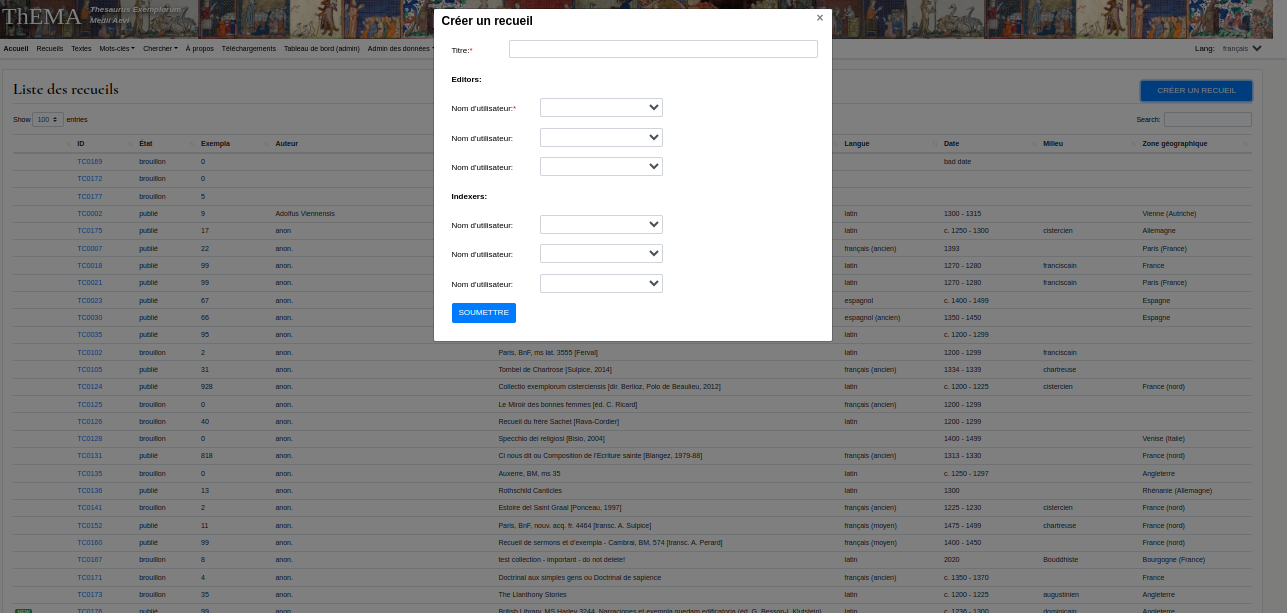
\includegraphics[width=0.6\linewidth]{images/creerrecueil.png}}
		\caption{Créer un recueil}
	\end{figure}

\textbf{Modifier un recueil}
\begin{flushleft}	
	- Se rendre dans la liste des recueils et en sélectionner un \\
	- Cliquer sur « Modifier » \\
	- Attendre la fin du chargement \\
	- Remplir les champs \\
	- Si les volets déroulant ne contiennent pas les informations nécessaires il faut se rendre dans « Admin des données » et les ajouter \\
\end{flushleft}	

	\begin{figure}[H]
	\centering
	\fbox{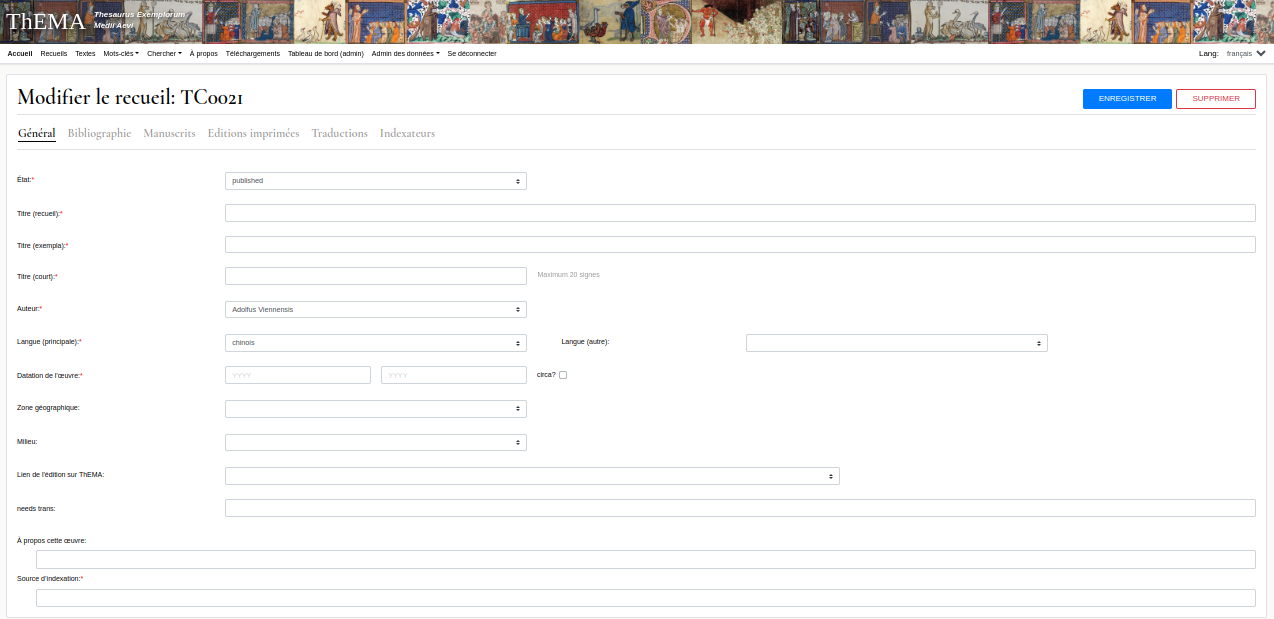
\includegraphics[width=0.6\linewidth]{images/creerrecueill.png}}
	\caption{Modifier un recueil}
	\end{figure}
	
\textbf{Créer ou modifier un \textit{exemplum}}
\begin{flushleft}	
	- Se rendre dans le tableau de bord ou dans le recueil créé \\
	- Cliquer sur « Créer un \textit{exemplum} \\
	- Attendre la fin du chargement \\
	- Compléter les champs \\
	- Si les volets déroulant ne contiennent pas les informations nécessaires il faut se rendre dans « Admin des données » et les ajouter \\
	- Enregistrer les modifications avec le bouton vert en haut à droite \\
	- Pour supprimer un \textit{exemplum} appuyer sur le bouton rouge « supprimer » \\
\end{flushleft}	
	
\begin{figure}[H]
	\centering
	\fbox{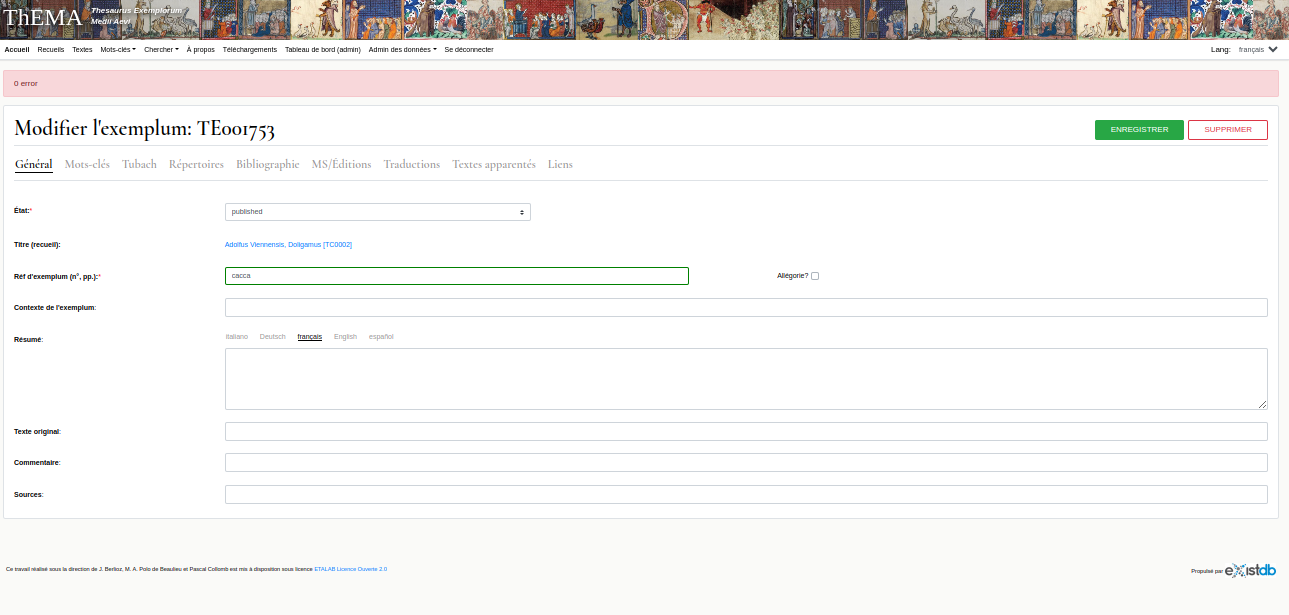
\includegraphics[width=0.6\linewidth]{images/creerexemplum.png}}
	\caption{Créer un \textit{exemplum}}
\end{figure}